\newcommand{\sets}{\mathbf{Sets}}
\newcommand{\op}[1]{{#1}^{\mathrm{op}}}
\newcommand{\arr}[1]{{#1}^{\rightarrow}}
\section{Categories}\cite{awodey}
\subsection{Foundations}
\DEF{Category,category}
A \EMPH{category} consists of the followings:
\begin{itemize}
\item \EMPH{Objects} $A$, $B$, $C, \dotsc$
\item \EMPH{Arrows} $f$, $g$, $h, \dotsc$ with the objects called the domain $\dom f$ and the codomain $\cod f$.
\item \EMPH{Composites} $g \circ f \colon A \to C$ for given arrows $f \colon A \to B$ and $g \colon B \to C$.
\item \EMPH{Identity arrow} $1_A$ of each object $A$.
\end{itemize}
satisfying the following laws:
\begin{enumerate}
\item $\forall \text{arrows}\ f \colon A \to B, g \colon B \to C, h \colon C \to D,\ h \circ (g \circ f) = (h \circ g) \circ f$
\item $\forall \text{arrow}\ f \colon A \to B,\ f \circ 1_A = f = 1_B \circ f$.
\end{enumerate}

\DEF{Functor between categories,functor-between-categories}
A \EMPH{functor} $F\colon \s A \to \s B$ between categories $\s A$ and $\s B$ is a mapping between objects and between arrows in the following ways:
\begin{enumerate}
\item $F(f\colon A \to B) = F(f) \colon F(A) \to F(B)$,
\item $F(1_A) = 1_{F(A)}$,
\item $F(g \circ f) = F(g) \circ F(f)$.
\end{enumerate}

\DEF{Isomorphism between categories,isomorphism-between-categories}
In a category $\s C$, an arrow $f \colon A \to B$ is called an \EMPH{isomorphism} if
\[
\exists g = f^{-1} \colon B \to A,\ g \circ f = 1_A,\ f \circ g = 1_B.
\]
If there is an isomorphism between objects $A$ and $B$, $A$ is said to be \EMPH{isomorphic} to $B$, written $A \cong B$.

\THM{Category is isomorphic to its Cayley representation,category-is-isomorphic-to-its-cayley-representation}
For a category $\s C$ with a set of arrows, the Cayley representation $\BAR{\s C}$ of $\s C$, consisting of
\begin{itemize}
  \item object $\BAR C = \{ f \in \s C \mid \cod f = C \}$ for an object $C \in \s C$,
  \item arrow $\BAR g \colon \BAR C \to \BAR D$ for an arrow $g \colon C \to D$ such that $\BAR g (f) = g \circ f$,
\end{itemize}
is isomorphic to $\s C$.

\DEF{Product of two categories,product-of-two-categories}
The \EMPH{product} $\s C \times \s D$ of categories $\s C$ and $\s D$ consists of
\begin{itemize}
  \item object $ (C, D)$ for objects $C \in \s C$, $D \in \s D$,
  \item arrow $(f, g) \colon (C, D) \to (C', D')$ for arrows $f \colon C \to C'$, $g \colon D \to D'$,
\end{itemize}
with composition $(f, g) \circ (f', g') = (f \circ f', g \circ g')$ and units $1_{(C,D)} = (1_C, 1_D)$.

The \EMPH{projection functors} $\pi_1 \colon \s C \times \s D \to \s C$ and $\pi_2 \colon \s C \times \s D \to \s D$ is defined by $\pi_1 (C, D) = C$ and $\pi_1 (f,g) = f$, and similarly for $\pi_2$.

\DEF{Dual category,dual-category}
For a category $\s C$, its \EMPH{dual} or \EMPH{opposite category} $\op{\s C}$ consists of
\begin{itemize}
  \item object $C^* = C$ for an object $C \in \s C$,
  \item arrow $f^* \colon D^* \to C^*$ for an arrow $f \colon C \to D$,
\end{itemize}
with composition $f^* \circ g^* = ( g \circ f)^*$ and units $1_{C^*} = (1_C)^*$.
\par\quad
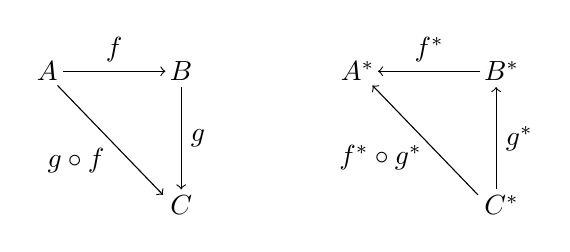
\begin{tikzpicture}
\node at(0,0) {$A$};
\draw[->] (.2,0) -- (1.5,0);
\node at(1.7,0) {$B$};
\node[above] at(.85,0) {$f$};
\draw[->] (1.7,-.2) -- (1.7,-1.5);
\node at(1.7,-1.7) {$C$};
\node[right] at(1.7,-.85) {$g$};
\draw[->] (.13,-.18) -- (1.47,-1.57);
\node[below left] at(.85,-.85) {$g \circ f$};
\node at(3.94,0) {$A^*$};
\draw[->] (5.5,0) -- (4.2,0);
\node at(5.77,0) {$B^*$};
\node[above] at(4.85,0) {$f^*$};
\draw[->] (5.7, -1.5) -- (5.7,-.2);
\node at(5.77,-1.7) {$C^*$};
\node[right] at(5.7,-.85) {$g^*$};
\draw[->] (5.47, -1.57) -- (4.13,-.18);
\node[below left] at(4.88, -.82) {$f^* \circ g^*$};
\end{tikzpicture}

\DEF{Arrow category,arrow-category}
For a category $\s C$, its \EMPH{arrow category} $\arr{\s C}$ consists of
\begin{itemize}
  \item object $f \colon C \to D$ for an arrow $f$ in $\s C$,
  \item arrow $(g_1, g_2) \colon f \to f'$, where $f \colon A \to B, f' \colon A' \to B', g_1 \colon A \to A', g_2 \colon B \to B'$ in $\s C$, such that $g_2 \circ f = f' \circ g_1$,
\end{itemize}
with composition $(g_1, g_2) \circ (h_1, h_2) = (g_1 \circ h_1, g_2 \circ h_2)$ and units $1_f = (1_A, 1_B)$.
\par\quad
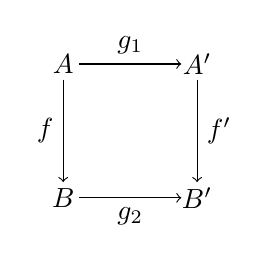
\begin{tikzpicture}
\node at(0,0) {$B$};
\draw[->] (.2,0) -- (1.5,0);
\node at(1.7,0) {$B'$};
\draw[->] (0,1.5) -- (0,.2);
\draw[->] (1.7,1.5) -- (1.7,.2);
\node at(0,1.7) {$A$};
\node at(1.7,1.7) {$A'$};
\draw[->] (.2,1.7) -- (1.5,1.7);
\node[below] at(.85,0) {$g_2$};
\node[left] at(0,.85) {$f$};
\node[right] at(1.7,.85) {$f'$};
\node[above] at(.85,1.7) {$g_1$};
\end{tikzpicture}

There are two functors $\dom, \cod \colon \arr{\s C} \to \s C$.

\DEF{Slice category,slice-category}
For a category $\s C$, its \EMPH{slice category} $\s C/C$ over $C \in \s C$ consists of
\begin{itemize}
  \item object $f \colon X \to C$,
  \item arrow $a \colon X \to X'$ for arrows $f \colon X \to C, f' \colon X' \to C$ such that $f' \circ a = f$,
\end{itemize}
with composition and units from those of $\s C$.
\newline\quad
\begin{tikzpicture}
\node at(0,0) {$X$};
\draw[->] (.2,0) -- (3.8,0);
\node at(4,0) {$X'$};
\draw[->] (.18,-.2) -- (1.8,-1.5);
\node at(1.92,-1.7) {$C$};
\draw[->] (3.83, -.2) -- (2.1,-1.5);
\node[above] at(2,0) {$a$};
\node[below left] at(1.03,-.865) {$f$};
\node[below right] at(2.85,-.87) {$f'$};
\end{tikzpicture}

$U \colon \s C/C \to \s C$ with $U(f \colon X \to C) = X$ and $U(a \colon X \to X') = a$ is a functor.
